\documentclass[10pt,a4paper]{article}
\usepackage[slovak]{babel}
\usepackage[utf8]{inputenc}
\usepackage{amsmath}
\usepackage{amsfonts}
\usepackage{amssymb}
\usepackage[unicode]{hyperref}
\usepackage{graphicx}

\textwidth 6.5in
\oddsidemargin 0.0in
\evensidemargin 0.0in

\title{Poznámky z Úvodu do diskrétnych štruktúr - materiál na štátnice}
\date{18.06.2012}
\author{Peter Csiba, petherz@gmail.com, \url{https://github.com/Petrzlen/fmfi-poznamky/diskretka/}} 

\begin{document}
\maketitle
\tableofcontents

\clearpage

%%%%%%%%%%%%%%%%%%%%%%%%%%%%%%%%%%%%%%%%%%%%%%%%%%%%%%%%%%%%%%%%%%%%%%%%%%%%%%%%
%%%%%%%%%%%%%%%%%%%%%%%%%%%%%%%%%%%%%%%%%%%%%%%%%%%%%%%%%%%%%%%%%%%%%%%%%%%%%%%%
\section*{Úvod}   

Tento text vysvetľuje netriviálne a nejasné pasáže z predmetu Úvod do diskrétnej matematiky,
prípadne patchuje chyby v skriptách. 

Autor si v matematike a hlavne jej diskrétnej a kombinatorickej časti naozaj verí. 

Nakoniec poznamenajme, že autor sa snažil písať pravdu a len pravdu, keďže jeho odpoveď na záverečných skúškach vychádza z tototo materiálu.
Ak čitateľ chce prispieť ku kvalite textu, nech autorovi napíše a ten mu udelí prístup do repozitára.

\clearpage

%%%%%%%%%%%%%%%%%%%%%%%%%%%%%%%%%%%%%%%%%%%%%%%%%%%%%%%%%%%%%%%%%%%%%%%%%%%%%%%%
%%%%%%%%%%%%%%%%%%%%%%%%%%%%%%%%%%%%%%%%%%%%%%%%%%%%%%%%%%%%%%%%%%%%%%%%%%%%%%%%
\section{Cantor-Bernstein}   

Po analýze dôkazu z Olejár-Škoviera sme dospeli k jednoznačnému názoru, že je tam chyba (resp. preklep). Dôkaz vystihujúci podstatu je možné nájsť na \href{http://en.wikipedia.org/wiki/Cantor\%E2\%80\%93Bernstein\%E2\%80\%93Schroeder_theorem}{Wikipédií}. Ja som sa snažil formulovať čo najnázornejšie. 

\paragraph{Veta.} Nech sú $A$ a $B$ ľubovoľné množiny a nech existujú injektívne zobrazenia $f : A \mapsto B$ a $g : B \mapsto A$. Potom množiny $A$ a $B$ majú rovnakú mohutnosť. 

\paragraph{Dôkaz.} Ku každému prvku $a \in A$ priradíme nasledujúcu postupnosť
$$
(\ldots, g^{-1}(f^{-1}(g^{-1}(a))), f^{-1}(g^{-1}(a)), g^{-1}(a), a, f(a), g(f(a)), \ldots),
$$
ktorú nazveme \emph{reťazou} pre $a$. Prvky vľavo od $a$ nazveme \emph{predkami} $a$ a vpravo \emph{potomkami} $a$. Všimnime si, že $a$ má vždy nekonečno potomkov (môžu sa opakovať). Na druhej strane, môže sa stať, že $a$ má iba konečný počet predkov. Určite si to skúste nakresliť ako dve množiny $A$ a $B$ s prvkami a šípkami reprezentujúce $f$ a $g$ (potom vlastne hľadáme párovanie množiny vrcholov, tj. bijekciu).

Reťaze sú troch \underline{disjunktných} typov. Nemajú prvý prvok (nekonečné, resp. cyklické), alebo začínajú v $A$, alebo začínajú v $B$. Definujeme funkciu $h : A \mapsto B$ pre každé $a \in A$ nasledovne 
\begin{itemize}
\item $h(a) = f(a)$, ak reťaz prislúchajúca k $a$ a začína v $A$
\item $h(a) = g^{-1}(a)$, ak reťaz prislúchajúca k $a$ a začína v $B$
\item $h(a) = f(a)$, ak má $a$ nekonečno veľa predkov. 
\end{itemize}

Tvrdíme, že $h$ je bijektívne zobrazenie. Je zrejmé, že je dobre definované (každý prvok má iba jeden obraz). Je injektívne, lebo keby $h(a)=h(b) \wedge a \neq b (a,b \in A)$, tak by $a$ a $b$ museli mať rôzne typy reťazí, a teda 
$$
f(a)=h(a)=h(b)=g^{-1}(b).
$$
Potom ale $a, f(a), b$ sú v spoločnej reťazi v tomto poradí, čo je spor s definíciou $h$ (prepokladaly sme rôzne typy reťazí, ale sú rovnaké). Surjektívne je preto, lebo ak uvažujeme reťaz pre každý prvok $b \in B$ (s podobnou definíciou reťaze pre $B$), tak k nej existuje rovnaká reťaz nejakého prvku $a \in A$. Keďže sme všetky reťaze pre $a \in A$ spárovali (ako na obrázku), tak sme nevynechali žiadne $b$ z oboru hodnôt. 

\begin{center}
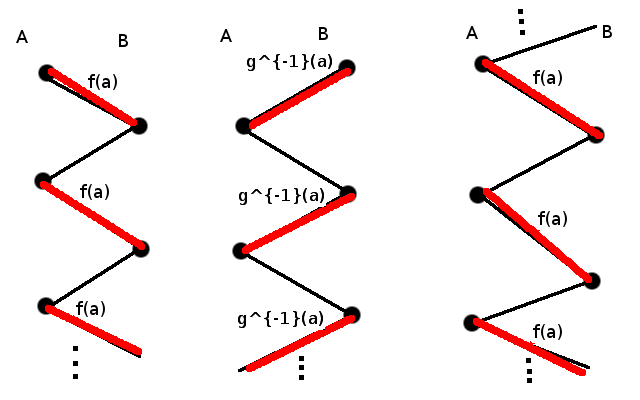
\includegraphics[scale=0.5]{parovanie.png}
\end{center}



%%%%%%%%%%%%%%%%%%%%%%%%%%%%%%%%%%%%%%%%%%%%%%%%%%%%%%%%%%%%%%%%%%%%%%%%%%%%%%%%
%%%%%%%%%%%%%%%%%%%%%%%%%%%%%%%%%%%%%%%%%%%%%%%%%%%%%%%%%%%%%%%%%%%%%%%%%%%%%%%%
\clearpage
\section*{Referencie a odporúčaná literatúra}
Obe skriptá sú v repozitáry. 

\begin{itemize}                                
\item Úvod do diskrétnych matematických štruktúr. Daniel Olejár a Martin Škoviera.
\item Úvod do diskrétnych štruktúr. Eduard Toman, BRATISLAVA 2008.
\end{itemize}

\end{document}
